\documentclass[11pt,a4paper]{article}

% ---------- FONTS & ENCODING ----------
\usepackage{fontspec}
\setmainfont{TeX Gyre Pagella}
\setsansfont{TeX Gyre Heros}

% ---------- LAYOUT & PACKAGES ----------
\usepackage[a4paper,top=2.3cm,bottom=2.3cm,left=2.6cm,right=2.6cm]{geometry}
\usepackage[table]{xcolor}
\usepackage{graphicx}
\usepackage{tikz}
\usetikzlibrary{shapes.geometric, arrows.meta, positioning}
\usepackage{titlesec}
\usepackage{tcolorbox}
\tcbuselibrary{skins,breakable}
\usepackage{booktabs}
\usepackage{array}
\usepackage{longtable}
\usepackage{enumitem}
\usepackage{fancyhdr}
\usepackage{hyperref}
\usepackage{ragged2e}
\usepackage{xstring}
\usepackage{setspace}
\usepackage{pgfgantt} 

% ---------- BRAND COLORS (Palette A: Navy & Amber) ----------
\definecolor{navy}{HTML}{1B2A6B}
\definecolor{navydark}{HTML}{10193F}
\definecolor{amber}{HTML}{F2994A}
\definecolor{ink}{HTML}{1A1A1A}
\definecolor{softgray}{HTML}{6E6E6E}
\definecolor{mutedblue}{HTML}{9AA6CE}
\definecolor{linegray}{HTML}{E7E7E7}
\definecolor{tabletint}{HTML}{F8F9FC} 

\hypersetup{colorlinks=true, linkcolor=ink, urlcolor=navy}

% ---------- SECTION STYLE (High-End Agency Design) ----------
\titleformat{\section}
  {\normalfont\bfseries\fontsize{19}{24}\selectfont\color{navydark}}
  {\textcolor{amber}{\fontsize{24}{24}\selectfont\thesection}\hspace{0.5em}\textcolor{linegray}{\rule[-2pt]{1.5pt}{18pt}}\hspace{0.2em}}
  {0em}
  {}
  [\vspace{6pt}\rlap{\textcolor{amber}{\rule{2.5cm}{1.5pt}}}\textcolor{linegray}{\rule{\linewidth}{0.5pt}}]
\titlespacing*{\section}{0pt}{2.4em}{1.2em}

% Subsection: Clean matching Amber number
\titleformat{\subsection}
  {\normalfont\bfseries\fontsize{13}{16}\selectfont\color{navy}}
  {\textcolor{amber}{\thesubsection}}
  {0.8em}
  {}
\titlespacing*{\subsection}{0pt}{2em}{1em}

% ---------- HEADER / FOOTER (single hairline, minimal) ----------
\pagestyle{fancy}
\fancyhf{}
\renewcommand{\headrulewidth}{0pt}
\renewcommand{\footrulewidth}{0pt}
\fancyhead[L]{\fontsize{7.6}{10}\selectfont\color{softgray}\textsc{Agam AI Labs}}
\fancyhead[R]{\fontsize{7.6}{10}\selectfont\color{softgray}\textsc{Synthetic Monitoring -- BRD}}
\fancyfoot[L]{\fontsize{7.6}{10}\selectfont\color{softgray}\textsc{Confidential}}
\fancyfoot[R]{\fontsize{7.6}{10}\selectfont\color{amber}\thepage}
\renewcommand{\headrule}{{\color{linegray}\hrule height 0.6pt}}


% =====================================================
% ---------- UI/UX ELEMENTS: BRAND-ALIGNED CHIPS ----------
% =====================================================

\newtcbox{\uibadge}[3][navy]{on line, arc=2.5pt, colback=#2, colframe=#1, boxrule=0.5pt,
  fontupper=\bfseries\sffamily\fontsize{7.5}{7.5}\selectfont,
  colupper=#3, boxsep=0pt, left=6pt, right=6pt, top=3pt, bottom=3pt}

\newcommand{\severity}[1]{%
  \ifstrequal{#1}{High}{\uibadge[navydark]{navydark}{white}{High priority}}{%
  \ifstrequal{#1}{Medium}{\uibadge[amber]{amber!15}{navydark}{Medium priority}}{%
  \uibadge[mutedblue]{mutedblue!15}{navydark}{Low priority}}}%
}

\newcommand{\pri}[1]{%
  \ifstrequal{#1}{High}{\uibadge[navydark]{navydark}{white}{High}}{%
  \ifstrequal{#1}{Medium}{\uibadge[amber]{amber!15}{navydark}{Medium}}{%
  \uibadge[mutedblue]{mutedblue!15}{navydark}{Low}}}%
}

\newcommand{\thd}[1]{\textsc{\bfseries\color{white}\fontsize{8.6}{8.6}\selectfont #1}}


% =====================================================
% ---------- CALLOUT BLOCKS (Sharp Modern Shadows & Mini-Chips) ----------
% =====================================================

\newtcolorbox{issuebox}[2]{
  enhanced, colback=white, colframe=linegray, boxrule=0.5pt,
  borderline west={4pt}{0pt}{navy}, 
  arc=2pt, outer arc=2pt, breakable, 
  top=14pt, bottom=14pt, left=16pt, right=16pt,
  before skip=18pt, after skip=18pt,
  shadow={3pt}{-3pt}{0pt}{navy!10}, 
  before upper={%
    \tcbox[on line, boxsep=0pt, boxrule=0pt, colback=navy!8, colframe=navy!8, left=5pt, right=5pt, top=3pt, bottom=3pt, arc=2pt]{\sffamily\bfseries\fontsize{8}{10}\selectfont\color{navy}\MakeUppercase{#1}}\\[8pt]
    {\bfseries\fontsize{14}{16}\selectfont\color{navydark}#2}\\[6pt]
    {\color{linegray}\hrule height 0.5pt}\vspace{10pt}
  }
}

\newtcolorbox{recbox}[2]{
  enhanced, colback=white, colframe=linegray, boxrule=0.5pt,
  borderline west={4pt}{0pt}{amber}, 
  arc=2pt, outer arc=2pt, breakable, 
  top=14pt, bottom=14pt, left=16pt, right=16pt,
  before skip=18pt, after skip=18pt,
  shadow={3pt}{-3pt}{0pt}{amber!15}, 
  before upper={%
    \tcbox[on line, boxsep=0pt, boxrule=0pt, colback=amber!15, colframe=amber!15, left=5pt, right=5pt, top=3pt, bottom=3pt, arc=2pt]{\sffamily\bfseries\fontsize{8}{10}\selectfont\color{amber!90!black}\MakeUppercase{#1}}\\[8pt]
    {\bfseries\fontsize{14}{16}\selectfont\color{navydark}#2}\\[6pt]
    {\color{linegray}\hrule height 0.5pt}\vspace{10pt}
  }
}

% --- CUSTOM VALUE CARDS (3-COLUMN GRID) ---
\newtcolorbox{valuecard}[1]{
  enhanced, colback=white, colframe=linegray, boxrule=0.5pt,
  borderline north={3pt}{0pt}{navy}, 
  width=0.31\textwidth, nobeforeafter,
  arc=2pt, top=14pt, bottom=14pt, left=10pt, right=10pt,
  shadow={2pt}{-2pt}{0pt}{navy!4},
  before upper={%
    \centering\sffamily\bfseries\fontsize{10.5}{12}\selectfont\color{amber}\MakeUppercase{#1}\\[6pt]
    {\color{linegray}\hrule height 0.5pt}\vspace{8pt}%
    \normalfont\fontsize{9.5}{13}\selectfont\color{navydark}%
  },
  after upper={}
}

\setlist[itemize]{label=\textcolor{amber}{\rule{3.5pt}{3.5pt}}, leftmargin=1.8em, itemsep=7pt, topsep=8pt}
\setlist[enumerate]{label=\textbf{\textcolor{navy}{\arabic*.}}, leftmargin=1.8em, itemsep=7pt, topsep=8pt}
\setstretch{1.18}
\arrayrulecolor{linegray}

% =====================================================
\begin{document}

% ================= COVER PAGE =================
\begin{titlepage}
\newgeometry{margin=0cm}
\begingroup
\pagecolor{navy}
\color{white}

\begin{tikzpicture}[remember picture, overlay]
  \fill[navy] (current page.north west) rectangle (current page.south east);

  \draw[amber!55, line width=0.9pt]
     ([xshift=-2cm,yshift=1.5cm]current page.south west) to[out=70,in=200]
     ([xshift=4cm,yshift=9cm]current page.south west) to[out=20,in=250]
     (current page.north east);
  \draw[mutedblue, line width=0.5pt, opacity=0.35]
     ([xshift=1cm,yshift=0cm]current page.south west) to[out=75,in=205]
     ([xshift=6cm,yshift=10.5cm]current page.south west) to[out=25,in=250]
     ([xshift=-1cm]current page.north east);

  \node[anchor=north west, fill=white, rounded corners=3pt, inner sep=9pt]
     at ([xshift=2.6cm,yshift=-2.6cm]current page.north west)
     {
\includegraphics[width=2.3cm]{../../Images/sarva.png}}; % Ensure logo path is correct

  \draw[amber, line width=1.6pt]
     ([xshift=2.6cm,yshift=-11.6cm]current page.north west) --
     ([xshift=2.6cm,yshift=-17.9cm]current page.north west);

  \node[anchor=north west, text=amber] at ([xshift=3.15cm,yshift=-11.9cm]current page.north west)
     {\fontsize{10.5}{13}\selectfont\textsc{COMMERCIAL \& PRODUCT ROADMAP PROPOSAL}};

  \node[anchor=north west, text=white, align=left, text width=13.8cm]
     at ([xshift=3.15cm,yshift=-13.1cm]current page.north west)
     {\fontsize{33}{39}\selectfont\bfseries AI-Powered Synthetic \\ Monitoring System};

  \node[anchor=north west, text=mutedblue, align=left, text width=11.5cm]
     at ([xshift=3.15cm,yshift=-17.3cm]current page.north west)
     {\fontsize{11.5}{16}\selectfont A phased monitoring platform roadmap, starting with Phase 1 and evolving toward multi-tenant SaaS and enterprise self-service.};

  \node[anchor=south west, text=mutedblue, align=left, text width=15.8cm]
     at ([xshift=2.6cm,yshift=2.9cm]current page.south west)
     {\fontsize{9}{14}\selectfont\textsc{Prepared for} \ Sarva Creation \quad\textbullet\quad \textsc{Prepared by} \ Agam AI Labs \quad\textbullet\quad September 04, 2026};

  \node[anchor=south west, text=mutedblue] at ([xshift=2.6cm,yshift=1.5cm]current page.south west)
     {\fontsize{8}{10}\selectfont\textsc{Ref. AGAL-2026-ALLOCABS-SM-002.01 \ -- \ Client Draft}};

\end{tikzpicture}

\endgroup
\nopagecolor
\restoregeometry
\end{titlepage}

% ================= TABLE OF CONTENTS =================
\thispagestyle{empty}
\begin{center}

\includegraphics[width=2.6cm]{../../Images/sarva.png}
\end{center}
\vspace{0.6em}
\tableofcontents
\newpage

% ================= SECTION 1: EXECUTIVE SUMMARY =================
\section{Executive Summary}

\begin{issuebox}{The Immediate Need}{Centralized Visibility for Hostinger Infrastructure}
\noindent\textcolor{navy}{\textit{One place to see what is healthy, what needs attention, and what is down}}\par\vspace{4pt}
The proposed Phase 1 solution provides Sarva Creation with a dedicated monitoring command center for its agreed Hostinger websites. Instead of manually checking individual sites, authorized users gain a single operational view for availability, key metrics, active warnings, and critical outage notifications.
\end{issuebox}

\subsection{What Phase 1 Delivers}

% The 3-Column Value Cards
\begin{center}
\begin{valuecard}{See}
All agreed websites consolidated into a single, unified operational dashboard.
\end{valuecard}
\hfill
\begin{valuecard}{Detect}
Real-time availability, system health, performance metrics, and early warnings.
\end{valuecard}
\hfill
\begin{valuecard}{Respond}
Automated email alerts triggered the moment a monitored site becomes unavailable.
\end{valuecard}
\end{center}

\vspace{1.5em}

\begin{recbox}{Phase 1 Overview}{A Focused Production Release}
\begin{description}[
    leftmargin=0.26\linewidth,
    labelwidth=0.24\linewidth,
    labelindent=0pt,
    itemsep=8pt,
    font=\bfseries\color{navy}
]
  \item[Investment] INR 1,15,000
  \item[Delivery] Up to 1 month from receipt of advance, required access, and confirmed scope.
  \item[Primary Deliverable] A dedicated web-based monitoring dashboard with Hostinger connectivity and automated email outage alerts.
  \item[Access] Multiple authorized logins for one organization with predefined basic roles, deployed in one agreed production environment.
\end{description}
\end{recbox}

\subsection{Strategic Approach}
The initial release is deliberately narrow: establish a reliable production system immediately, validate the operating model, and avoid overloading the first engagement. Phase 2 and Phase 3 are designed as optional, independent engagements subject to separate written approval.\footnote{The commercial proposal explicitly states that each phase operates as an independent engagement.}


% ================= SECTION 2: PHASE 1 SOLUTION =================
\section{Phase 1 -- The Monitoring Solution}

\subsection{Architectural Flow}
\vspace{0.5em}
\begin{center}

\includegraphics[width=\textwidth]{Images/archi.png}
\end{center}
\vspace{1.5em}

\subsection{Included Capabilities}
\vspace{0.5em}

\renewcommand{\arraystretch}{1.7}
\noindent
\begin{longtable}{@{}>{\raggedright\arraybackslash}p{0.28\linewidth}p{0.72\linewidth}@{}}
\rowcolor{navy}
\thd{CAPABILITY} & \thd{CLIENT VALUE} \\
\midrule
\endhead % Repeats the styled header if it breaks across pages
\textbf{Central Dashboard} & A single operational pane of glass for all agreed websites and their real-time monitoring status. \\
\rowcolor{tabletint}
\textbf{Availability Monitoring} & Automated uptime tracking using existing Hostinger interfaces to instantly detect site unavailability. \\
\textbf{Health \& Metrics} & Vital performance metrics, active warnings, and system status surfaced in a clean, scannable format. \\
\rowcolor{tabletint}
\textbf{Email Notifications} & Automated alerts dispatched directly to configured recipients the moment an outage is detected. \\
\textbf{Multi-User Access} & Secure, concurrent access for multiple authorized team members within a unified company environment. \\
\rowcolor{tabletint}
\textbf{Predefined Roles} & Out-of-the-box \textbf{Administrator} and \textbf{Viewer} roles for practical, immediate access control. \\
\textbf{Deployment \& Handover} & End-to-end setup: initial configuration, functional testing, production deployment, and team orientation. \\
\bottomrule
\end{longtable}

\vspace{2em}

\begin{recbox}{Phase 1 Outcome}{A usable operating experience, not just a codebase}
\textbf{Delivered at Handover:}
\begin{itemize}
  \item Fully deployed and tested monitoring dashboard in a production environment.
  \item Integrated inventory of agreed Hostinger websites.
  \item Live tracking of system health, status, and available metrics.
  \item Pre-configured and tested email alerts for outage detection.
  \item Comprehensive user orientation and operational handover.
\end{itemize}
\end{recbox}

% ================= SECTION 3: ROADMAP =================
\section{Product Roadmap}

The product lifecycle is strategically divided into three business stages: establish a reliable monitoring baseline (Phase 1), productize into a scalable commercial SaaS offering (Phase 2), and finally, introduce enterprise-grade governance and self-service capabilities (Phase 3).

\vspace{1em}
\subsection{Strategic Trajectory}

\renewcommand{\arraystretch}{1.7}
\begin{tabular}{@{}>{\raggedright\arraybackslash}p{0.22\linewidth}>{\raggedright\arraybackslash}p{0.25\linewidth}p{0.45\linewidth}@{}}
\rowcolor{navy}
\thd{STAGE} & \thd{CORE PURPOSE} & \thd{CAPABILITY EXPANSION} \\
\midrule
\textbf{\textcolor{navy}{01 -- Monitor}} \newline \textit{(Current Scope)} & \textbf{Dedicated Hostinger Solution} & Single-organization environment, predefined basic roles, central health dashboard, key metrics, and email outage alerts. \\
\rowcolor{tabletint}
\textbf{\textcolor{navy}{02 -- Scale}} \newline \textit{(Future Phase)} & \textbf{Multi-Tenant SaaS} & Logical data separation for multiple customers, super-admin controls, centralized alerts, and multi-cloud integrations. \\
\textbf{\textcolor{navy}{03 -- Govern}} \newline \textit{(Future Phase)} & \textbf{Self-Service B2B Platform} & Client-managed onboarding, rich RBAC, audit trails, policy controls, and compliance-oriented reporting. \\
\bottomrule
\end{tabular}
\vspace{2em}

% --- PHASE 2 SUBSECTION ---
\subsection{Phase 2 -- Scale (Multi-Tenant SaaS)}
Phase 2 transforms the internal monitoring tool into a repeatable, commercial SaaS product. It shifts the architecture from a single-organization deployment to a secure multi-tenant environment, allowing Sarva Creation to manage multiple customer accounts with strict logical data separation. 

It also expands the monitoring engine to include native connectors for mainstream cloud providers such as AWS and Microsoft Azure, alongside the existing Hostinger integration.

\vspace{0.5em}
\begin{issuebox}{Phase 2 Connector Add-On}{Custom Provider R\&D}
Where a required cloud provider or hosting connector falls outside the agreed mainstream set, custom connector research and development is required. 
\begin{itemize}
  \item \textbf{Initial R\&D Investment:} Estimated at \textbf{INR 60,000} for the baseline research and API feasibility assessment.
  \item \textbf{Implementation:} Subsequent development is scoped dynamically based on the technical complexity and API limitations of the requested provider.
\end{itemize}
\end{issuebox}
\vspace{1em}

% --- PHASE 3 SUBSECTION ---
\subsection{Phase 3 -- Govern (Enterprise Self-Service)}
Phase 3 elevates the platform to an enterprise-grade standard, minimizing administrative overhead for the core team by introducing self-service capabilities. 

This phase focuses on organizational autonomy, allowing client teams to manage their own onboarding, configure custom alerting policies, and define granular Role-Based Access Control (RBAC). Furthermore, it introduces comprehensive audit trails and compliance-oriented reporting, satisfying the requirements of mature enterprise and developer teams.

% ================= SECTION 4: DELIVERY & COMMERCIALS =================
\clearpage
\section{Delivery, Investment \& Trust}

\subsection{Phase 1 Delivery Plan}
\vspace{0.5em}
\begin{center}
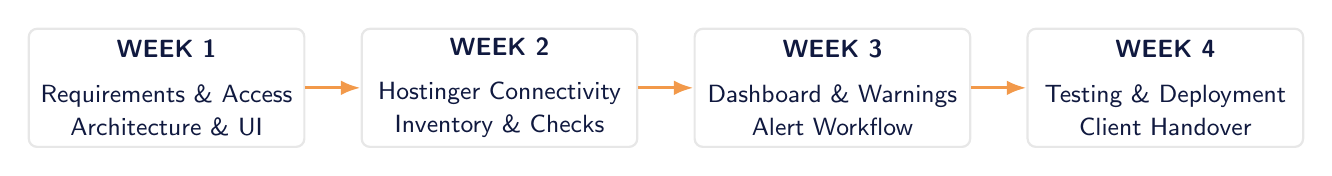
\begin{tikzpicture}[
  node distance=0.7cm, 
  box/.style={draw=linegray, line width=0.8pt, rounded corners=3pt, fill=white, minimum width=3.5cm, minimum height=1.5cm, align=center, text=navydark, font=\sffamily\fontsize{9}{12}\selectfont},
  arrow/.style={-{Latex[length=2.5mm]}, draw=amber, line width=1.2pt}
]
  \node[box] (w1) {\textbf{WEEK 1}\\[4pt] Requirements \& Access\\Architecture \& UI};
  \node[box, right=of w1] (w2) {\textbf{WEEK 2}\\[4pt] Hostinger Connectivity\\Inventory \& Checks};
  \node[box, right=of w2] (w3) {\textbf{WEEK 3}\\[4pt] Dashboard \& Warnings\\Alert Workflow};
  \node[box, right=of w3] (w4) {\textbf{WEEK 4}\\[4pt] Testing \& Deployment\\Client Handover};
  
  \draw[arrow] (w1) -- (w2);
  \draw[arrow] (w2) -- (w3);
  \draw[arrow] (w3) -- (w4);
\end{tikzpicture}
\end{center}
\vspace{1.5em}

\subsection{Commercial Snapshot}
\vspace{0.5em}
\begin{center}
\begin{valuecard}{Phase 1 Investment}
\textbf{INR 1,15,000}\\[4pt]
\textcolor{softgray}{\fontsize{8}{10}\selectfont (Exclusive of applicable taxes)}
\end{valuecard}
\hfill
\begin{valuecard}{Delivery Timeline}
\textbf{Up to 1 Month}\\[4pt]
\textcolor{softgray}{\fontsize{8}{10}\selectfont (From kickoff \& access grant)}
\end{valuecard}
\hfill
\begin{valuecard}{Primary Outcome}
\textbf{Live Dashboard}\\[4pt]
\textcolor{softgray}{\fontsize{8}{10}\selectfont (Monitoring engine \& alerts)}
\end{valuecard}
\end{center}
\vspace{1.5em}

\begin{recbox}{Controlled Execution}{Clear Outcomes, Firm Boundaries}
\begin{itemize}
  \item \textbf{Defined Release:} A fixed Phase 1 deliverable with a strict timeline, access model, and acceptance path.
  \item \textbf{Immediate Value:} Explicit focus on delivering monitored websites, the central dashboard, core metrics, and the alerting workflow.
  \item \textbf{Deferred Expansion:} Advanced SaaS capabilities, multi-tenant governance, and enterprise compliance remain safely segmented for future engagements.
\end{itemize}
\end{recbox}

\vspace{1em}
\subsection{Prerequisites \& Boundaries}
\vspace{0.5em}
\renewcommand{\arraystretch}{1.7}
\begin{tabular}{@{}>{\raggedright\arraybackslash}p{0.25\linewidth}p{0.75\linewidth}@{}}
\rowcolor{navy}
\thd{SCOPE CATEGORY} & \thd{PARAMETERS \& ASSUMPTIONS} \\
\midrule
\textbf{Client Inputs} & Authorized API/access credentials, finalized website inventory, alert recipient list, and designated technical contacts. \\
\rowcolor{tabletint}
\textbf{Monitoring Depth} & Relies strictly on the APIs, permissions, logs, and metrics externally available from Hostinger or connected providers. \\
\textbf{Phase 1 Boundary} & Deployed in one production environment with basic predefined roles. Advanced RBAC, mobile applications, custom reporting, or complex remediations require a separate quotation. \\
\rowcolor{tabletint}
\textbf{Operational Scope} & The platform provides visibility; it strictly excludes website repair, infrastructure administration, incident response services, or guaranteed prevention of downtime. \\
\bottomrule
\end{tabular}

\vspace{2.5em}
\subsection{Next Steps \& Project Initiation}
\vspace{0.5em}
\begin{center}

\begin{tikzpicture}[
  node distance=0.6cm, 
  stepstyle/.style={draw=linegray, line width=0.8pt, rounded corners=3pt, fill=white, minimum width=3.6cm, minimum height=0.9cm, align=center, text=navydark, font=\sffamily\bfseries\fontsize{8.5}{10}\selectfont}, 
  arrow/.style={-{Latex[length=2mm]}, draw=amber, line width=1.2pt}
]
  \node[stepstyle] (a) {1. Approve Phase 1};
  \node[stepstyle, right=of a] (b) {2. Confirm Inventory};
  \node[stepstyle, right=of b] (c) {3. Validate Access};
  \node[stepstyle, right=of c] (d) {4. Project Kickoff};
  
  \draw[arrow] (a) -- (b); 
  \draw[arrow] (b) -- (c); 
  \draw[arrow] (c) -- (d);
\end{tikzpicture}
\end{center}
\vspace{1em}

\noindent\textbf{Decision — Start with a focused first release.} 
Formal approval of this document confirms the website inventory, available Hostinger interfaces, alert thresholds, deployment arrangements, and acceptance criteria. Engineering commences immediately following the receipt of the agreed advance payment and required technical access.

\vfill
\noindent{\color{linegray}\rule{\linewidth}{0.6pt}}\\[6pt]
\fontsize{8.3}{10}\selectfont\textcolor{softgray}{Agam AI Labs \ -- \ Confidential. Prepared exclusively for Client Stakeholders.}

\end{document}